\section{Ejercicio 5}
\subsection{Introducci\'on}
\noindent
En el presente apartado se estudiar\'a el comportamiento y compatibilidad de dos compuertas l\'ogicas. Se utilizar\'a para ello una compuerta AND de tecnolog\'ia TTL y una compuerta OR de tecnolog\'ia CMOS. Inicialmente se analizar\'an sus respuestas individualmente y luego, de la forma en que se aprecia en la figura \ref{ej5_fig:compuertasjuntas}, se unir\'an la entrada de la OR-CMOS con la salida de la AND-TTL. A partir de esto, se observar\'an los nuevos resultados y se investigar\'an los distintos problemas que se pudieran presentar junto a sus posibles soluciones.

\begin{figure}[H]
    \centering
    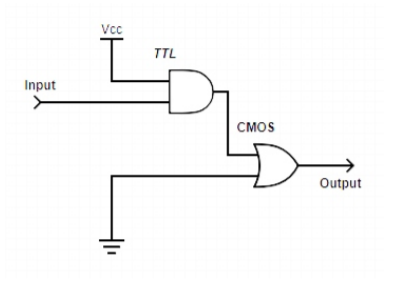
\includegraphics[scale=0.6]{figs/ej5/compuertas_juntas.png}
    \caption{Conexi\'on de las compuertas utilizadas.}
    \label{ej5_fig:compuertasjuntas}
\end{figure}

\subsection{An\'alisis previo}

\noindent
 Existen distintas consideraciones que deben realizarse cuando se interact\'ua entre las tecnolog\'ias a utilizar. En primer lugar, si se requiriera alimentar a integrados de ambas con una \'unica fuente, el rango posible de valores a utilizar se encuentra limitado por la tensi\'on aceptable de la tecnolog\'ia TTL, el cual se encuentra t\'ipicamente entre $4,75V$ y $5,25V$. 
 
\noindent
Luego, a modo de analizar la forma de realizar las correspondientes conexiones entre la salida de una tecnolog\'ia y la entrada de la otra, es necesario estudiar con que tensiones trabaja cada una en estos puntos. As\'i, en la figura \ref{ej5_fig:comparador_rangos} se detallan los valores alrededor de los cuales se encuentran los par\'ametros necesarios. Analizando lo que sucede al contar con una salida TTL y una entrada CMOS, se observa que $VOL_{TTL} < VIL_{CMOS}$ y que $VOH_{TTL} < VIH_{CMOS}$. Dado el primer caso (estado 0), no existen problemas por compatibilidad. No obtante, con respecto al segundo caso (estado 1), dado que la tensi\'on de salida en alto de una compuerta TTL puede ser menor que la tensi\'on en entrada en alto de una compuerta CMOS, \textbf{pueden presentarse problemas por incompatibilidad de tensi\'on}\label{ej5_ref:problema}.

\begin{figure}[H]
    \centering
    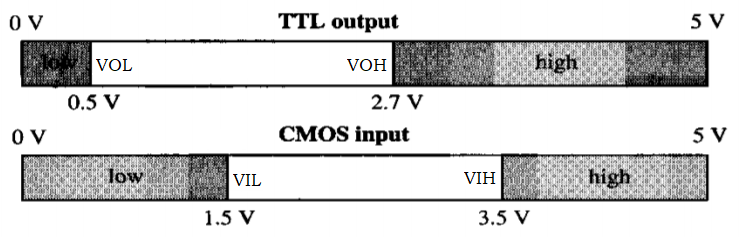
\includegraphics[scale=0.4]{figs/ej5/comparador_rangos_completo.png}
    \caption{Rangos de entrada y salida t\'ipicos de las tecnolog\'ias a utilizar.}
    \label{ej5_fig:comparador_rangos}
\end{figure}


\noindent
En adici\'on a la compatibilidad entre las tensiones, para la interconexi\'on de distintas tecnolog\'ias tambi\'en es necesario estudiar los requerimientos de corriente de cada una de ellas. Un factor de problem\'atica se da en el caso en que una compuerta de salida no pueda suministrar la corriente necesaria por la compuerta de entrada para interpretar un estado como tal. A partir de esto se detallan en la tabla \ref{ej5_tab:current_comparison} los valores de corriente con los que trabajan t\'ipicamente los integrados de tecnolog\'ia TTL y CMOS.

\begin{table}[H]
\centering
\begin{tabular}{ccc}
Par\'ametro & CMOS (74HC/HCT)     & TTL (74LS)   \\
IIH (min)      & $1\mu A$      & $20\mu A$  \\
IIL (min)      & $1\mu A$      & $0.6mA$ \\
IOH (m\'ax)      & $4mA$      & $0.4mA$ \\
IOL (m\'ax)      & $4mA$      & $8mA  $
\end{tabular}
\caption{Corrientes de entrada y salida de las tecnolog\'ias a utilizar.}
\label{ej5_tab:current_comparison}
\end{table}

\noindent
A partir de estas consideraciones, si se analiza la tabla \ref{ej5_tab:current_comparison} se concluye que \textbf{no existen problemas por incompatibilidad de corriente} al conectar la salida de una compuerta TTL con la entrada de una compuerta CMOS ya que las m\'aximas corrientes de salida son considerablemente mayores que las m\'inimas corrientes de entrada. A causa de esto, para el correcto funcionamiento del circuito no es necesario ajustar las corrientes pero si lo es introducir una etapa intermedia cuya funci\'on sea ajustar las tensiones para compatibilizar la salida y la entrada de los integrados a utilizar. A dichas etapas se las conoce como \textit{level shifters}. Esta debe asegurar que la tensi\'on de salida de la compuerta TTL sea mayor que la tensi\'on de entrada VIH de la compuerta CMOS. Para ello, existen distintas soluciones posibles.

\noindent
La primera de ellas es la incoporaci\'on de una resistencia entre ambas etapas de la forma mostrada en la figura \ref{ej5_fig:pull_up_res}. La presencia de esta resistencia ocasiona que la salida de la compuerta TTL aumente en estado alto su valor lo suficiente para conectarse correctamente con la compuerta subsiguiente.

\begin{figure}[H]
    \centering
    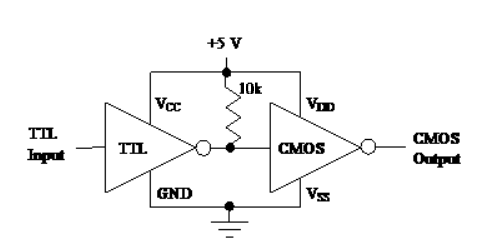
\includegraphics[scale=0.5]{figs/ej5/res_inter.png}
    \caption{Resistencia pull-up. Valor de referencia establecido en base a una alimentaci\'on com\'un de 5V (t\'ipica).}
    \label{ej5_fig:pull_up_res}
\end{figure}

\noindent
Otra posible soluci\'on es la utilizaci\'on de un integrado CD4504B\footnote{\href{https://www.ti.com/lit/ds/symlink/cd4504b-ep.pdf}{https://www.ti.com/lit/ds/symlink/cd4504b-ep.pdf}}, el cual se utiliza precisamente para estos casos, o el uso de un transistor BJT (permitiendo distintas alimentaciones) como se diagrama en la figura \ref{ej5_fig:transistor_inter}.

\begin{figure}[H]
    \centering
    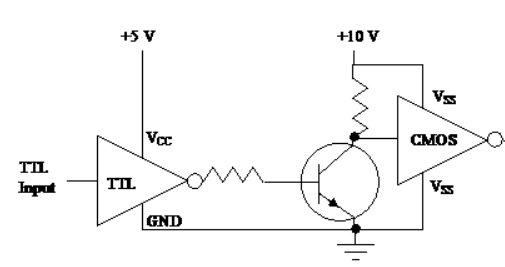
\includegraphics[scale=0.5]{figs/ej5/transistor_inter.png}
    \caption{Level Shifter mediante transistor NPN.}
    \label{ej5_fig:transistor_inter}
\end{figure}

\noindent
Existe otra soluci\'on interesante y es el caso del uso de un transistor BJT PNP entre ambas etapas, como se muestra en la figura \ref{ej5_fig:transistor_inter_pnp}. A su vez, otras posibles implementaciones incluyen transistores MOSFET o buffers TTL en la interconexi\'on. 

\begin{figure}[H]
    \centering
    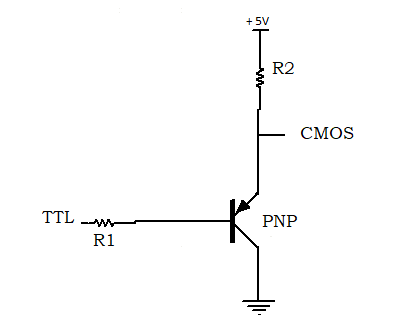
\includegraphics[scale=0.5]{figs/ej5/Levelshifter.png}
    \caption{Level Shifter mediante transistor PNP.}
    \label{ej5_fig:transistor_inter_pnp}
\end{figure}

\subsection{Implementaci\'on pr\'actica}
\noindent
Con el fin de llevar a cabo la presente experiencia, se decidi\'o utilizar un integrado digital 74LS08\footnote{\href{http://www.ti.com/lit/ds/symlink/sn74ls08.pdf}{http://www.ti.com/lit/ds/symlink/sn74ls08.pdf}} para la compuerta AND. Por su parte, para la compuerta OR se seleccion\'o un integrado digital 74HC32\footnote{\href{https://assets.nexperia.com/documents/data-sheet/74HC_HCT32.pdf}{https://assets.nexperia.com/documents/data-sheet/74HC_HCT32.pdf}}. En las respectivas hojas de datos se indica que la tensi\'on VOH m\'inima de la compuerta AND es de 2,4V y la VIH m\'inima de la compuerta OR es de 3,15V (con alimentaci\'on de 4,5V), pudiendo presentarse el problema ya descripto (ver \ref{ej5_ref:problema}).

\noindent
Como primera medida en la pr\'actica, se analizaron las salidas individuales de las compuertas encontr\'andose estas desconectadas entre s\'i. Para ello se aplicaron se\~nales cuadradas de 6Vpp a ambos bornes de entrada, generando valores de entrada altos y bajos alternadamente. Ante estas condiciones la salida deber\'ia tomar valores altos (tensi\'on mayor a VOH) y bajos (tensi\'on menor a VOL) respectivamente de acuerdo a la tensi\'on de entrada. En la figura \ref{ej5_fig:compuertas_desconectadas} se muestras las mediciones realizadas, ocurriendo efectivamente lo previsto.

\begin{figure}[H]
    \centering
    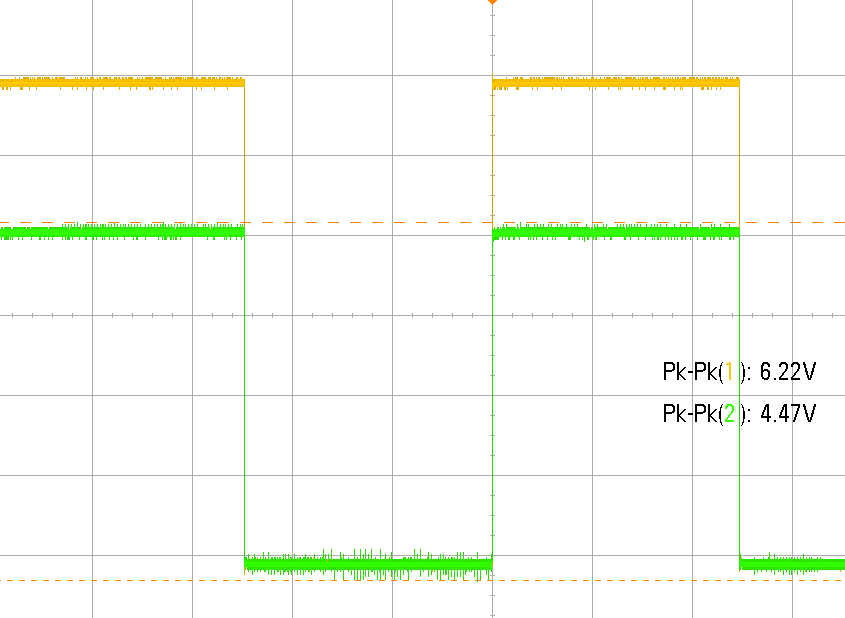
\includegraphics[width=.475\textwidth]{figs/ej5/and_cuadrada.png}\hfill
    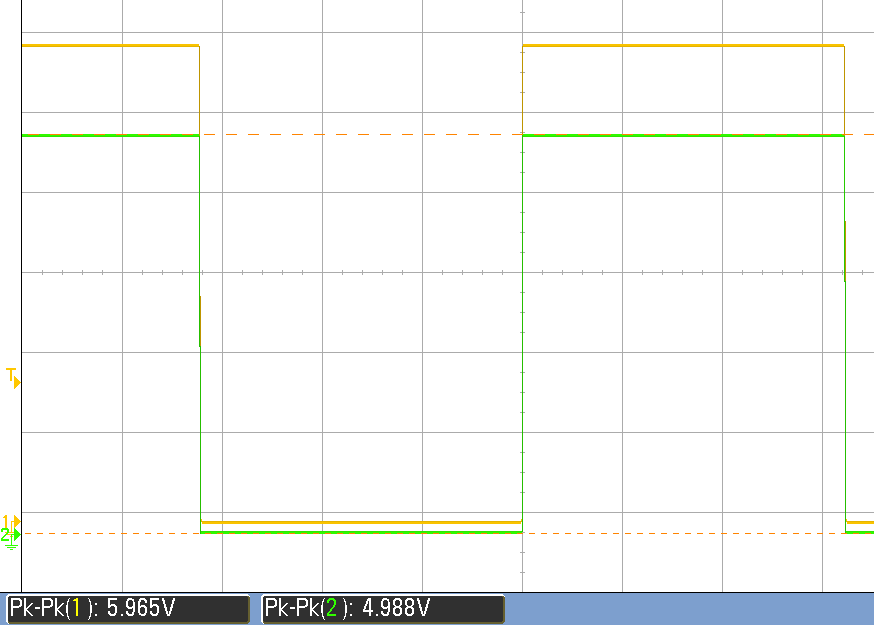
\includegraphics[width=.475\textwidth]{figs/ej5/or_cuadrada.png}
    \caption{Mediciones con las compuertas desconectadas.}
    \label{ej5_fig:compuertas_desconectadas}
    \subcaption{\footnotesize{*Izquierda: compuerta AND. Derecha: compuerta OR.}}
    \subcaption{\footnotesize{*Se\~nal amarilla: entrada. Se\~nal verde: salida.}}
\end{figure}

\noindent
Posteriormente, se realiz\'o el mismo procedimiento con las compuertas conectadas como en la figura \ref{ej5_fig:compuertasjuntas}. Al realizarlo, el circuito se comport\'o adecuadamente y no se registraron problemas por incompatibilidad. Sin embargo, bajo el prop\'osito de forzar su aparici\'on se carg\'o al circuito con una resistencia pull down entre ambas compuertas. Esto se realiz\'o ajustando el valor de un preset hasta que surgiera el error. Las mediciones se encuentran reflejadas en la figura \ref{ej5_fig:incompatibilidad}.

\begin{figure}[H]
    \centering
    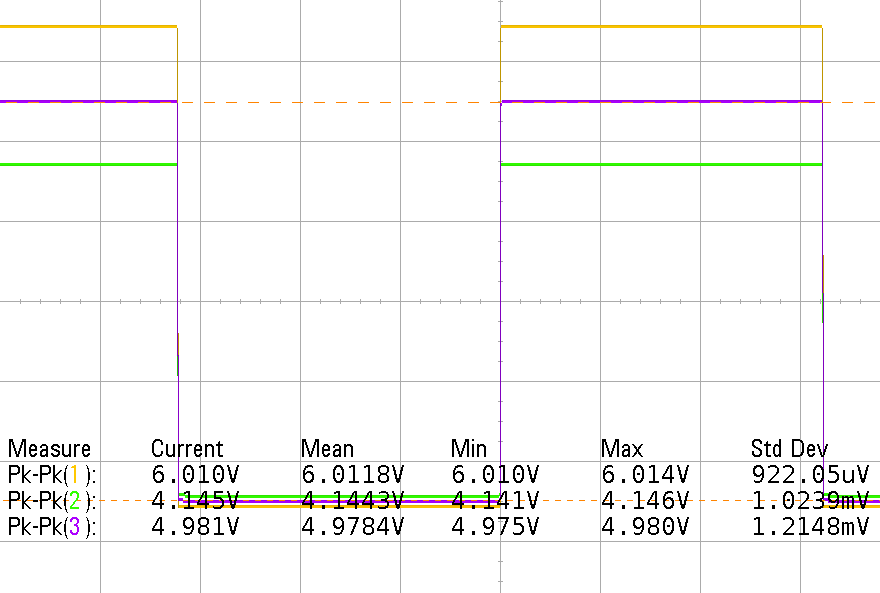
\includegraphics[width=.475\textwidth]{figs/ej5/andorsinres.png}\hfill
    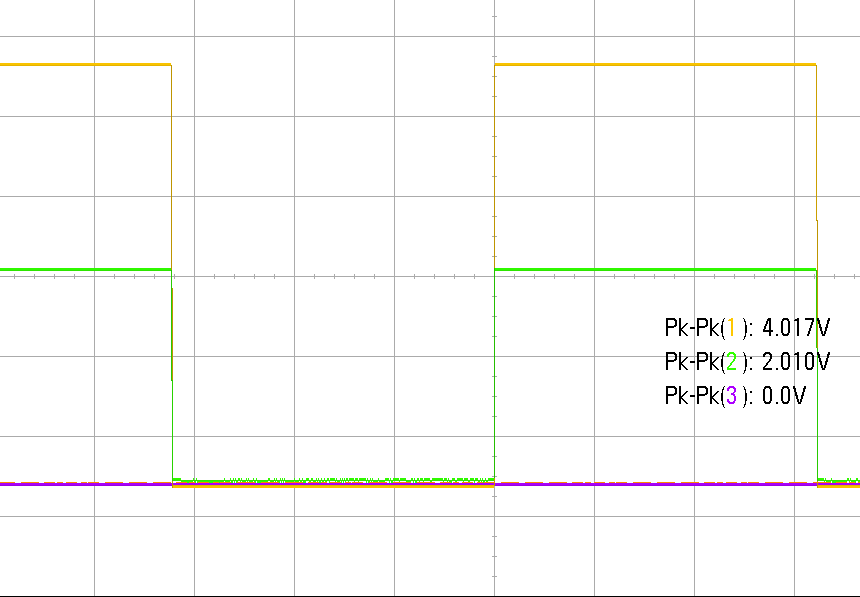
\includegraphics[width=.475\textwidth]{figs/ej5/pull_down.png}
    \caption{Mediciones con las compuertas conectadas.}
     \label{ej5_fig:incompatibilidad}
    \subcaption{\footnotesize{*Izquierda: respuesta del circuito. Derecha: incorporaci\'on de una carga.}}
    \subcaption{\footnotesize{*Se\~nal amarilla: entrada. Se\~nal violeta: etapa intermedia entre ambas compuertas. Se\~nal verde: salida.}}
   
\end{figure}

\noindent
Como soluci\'on ante dicho problema se incorpor\'o un level shifter mediante un transistor BJT PNP BC557 y dos resistores, de la forma diagramada en la figura \ref{ej5_fig:transistor_inter_pnp}, siendo R1 de 1k$\Omega$ y R2 de 10k$\Omega$. Esta etapa gener\'o un aumento en la tensi\'on de salida de la compuerta AND, resolviendo el problema de incompatibilidad. La salida en este caso se puede apreciar en la figura \ref{ej5_fig:pull_up}.

\begin{figure}[H]
    \centering
    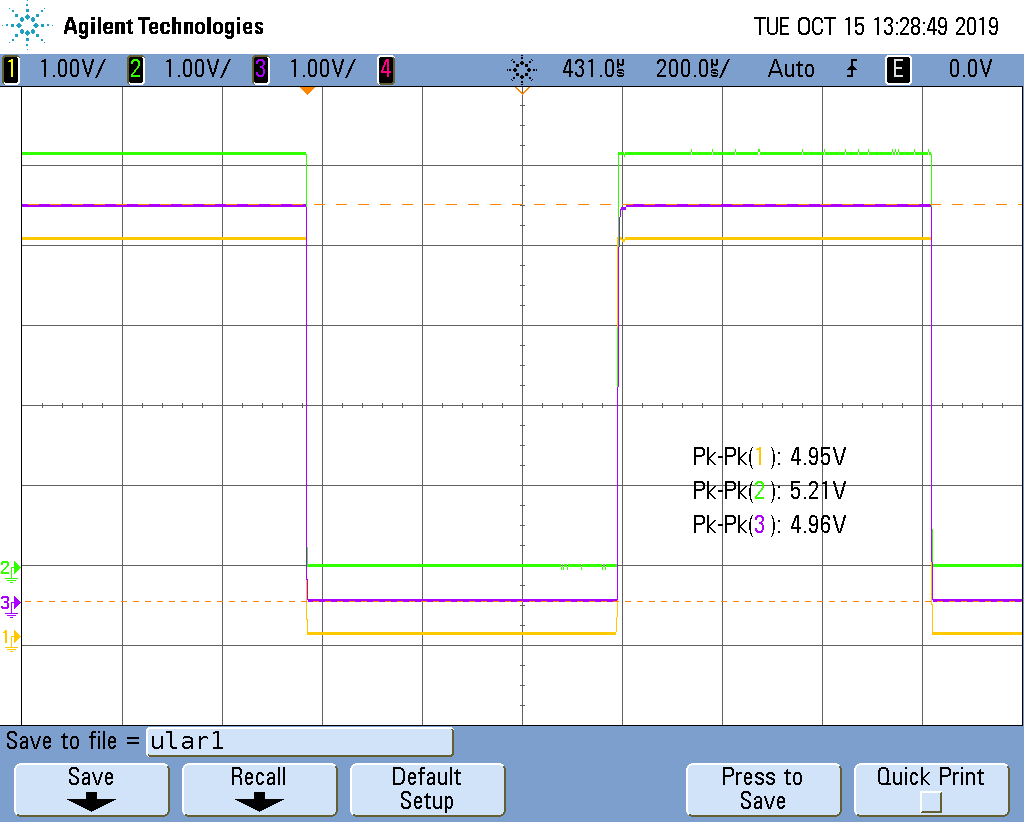
\includegraphics[width=0.6\textwidth]{figs/ej5/levelshifter10k1k.png}
    \caption{Resoluci\'on de la incompatibilidad mediante un level shifter.}
    \label{ej5_fig:pull_up}
\end{figure}
\subsection{Conclusiones}
\noindent
Mediante la presente experiencia, se analiz\'o la compatibilidad entre la conexi\'on de una salida TTL con una entrada CMOS. Se evidenci\'o que aunque en primera medida el circuito se comporte normalmente, pueden surgir problemas que son necesarios tener en cuenta.
\noindent
El problema mencionado se da por el hecho de que la tensi\'on de salida de una compuerta TTL puede ser menor que la tensi\'on VIH de una CMOS en estado alto. Con el fin de solucionar la problem\'atica, existen distintas opciones. En este caso, se incorpor\'o una etapa de lever shifting entre ambas compuertas, la cual di\'o lugar a un aumento de la tensi\'on de salida de la TTL, solventando el problema desarrollado.